\section{Convolution Experiments}
\label{cnn_predicts}

I decided to expand my dataset in a new way by 
using the image of a card as input to predict classes
of the card. Initially, this meant only using the art
to predict card color and type. The structure of my
network is very similar to the one mentioned before:
I feed in a vector (in this case the image) and output
a one--hot encoded result vector which indicates type
or color. These models trained with a batch size of 128
for about 20 epochs on 13,000 card images. The model
is shown in the appendix for clarity.

\subsection{Just the Art}
The final step I took in working on this project
was constructing a CNN to predict color and type
based on the image art alone. It is important to 
note that the image art is only the cropped art
as shown in figure \ref{fig:intro_card}.

The dataset of the art was constructed on my own
by crawling https://gatherer.wizards.com for card 
images and cropping them down to size\cite{gatherer}.
I then fed these images into a simple CNN with the 
following results:\\
Color Prediction: 35\%\\
Type Prediction: 53\%

The accuracy of the Color Prediction is shown in figure \ref{fig:cnn_results}.

\begin{figure}[h!]
    \centering
    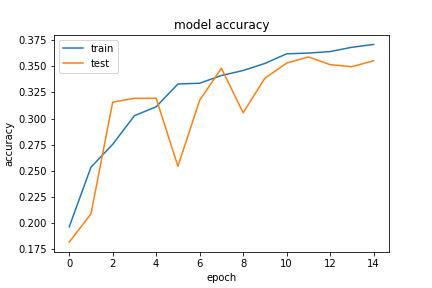
\includegraphics[width=0.8\linewidth]{figures/cnn_results.png} 
    \caption{Color Prediction Accuracy}
    \label{fig:cnn_results}
\end{figure}

\subsection{The Full Card}
After trying to work with just the image art and receiving
low results, I wanted a boost, so I included the entire image.
Obviously, I was expecting very high accuracies, because the 
color of a card is very clearly embedded in the image of the 
card itself. The type is also clear, but in text, which would 
be slightly more difficult to predict. Using the same 
architecture as the above experiments but with twice as many features
in each layer (eg. 256--256--128--128...).

My results are shown in the figure \ref{fig:full_color} and figure \ref{fig:full_type}.
\begin{figure}[h!]
    \centering
    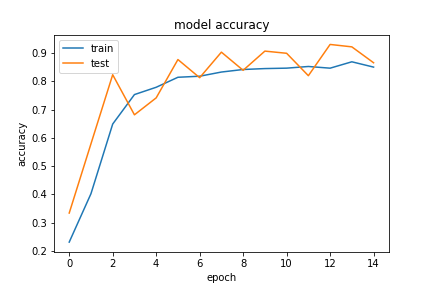
\includegraphics[width=0.8\linewidth]{figures/full_color.png} 
    \caption{Predict Color on Full Card Image}
    \label{fig:full_color}
\end{figure}

\begin{figure}[h!]
    \centering
    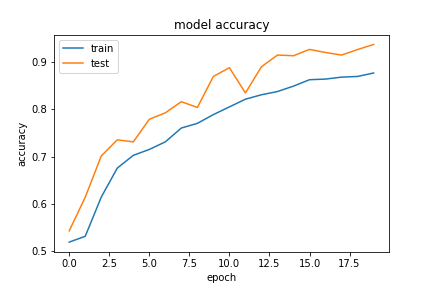
\includegraphics[width=0.8\linewidth]{figures/full_type.png} 
    \caption{Predict Type on Full Card Image}
    \label{fig:full_type}
\end{figure}

\subsection{Making Money}
The final experiments I ran were to test if I could predict the 
price of a card given the full image. This task presented new 
challenges primarily in the form of acquiring a dataset (as explained
in the bonus points section). I gathered my data from MtGGoldfish\cite{goldfish}.
Eventually I was able to train my CNN
on 15,000 card images and prices. I created buckets of prices at:
<\$0.15,<\$0.18,<\$0.25,<\$0.50,<\$1.50,<\$5.00, and above. These buckets
were all fairly evenly full at approximately 2,500 items each. The 
largest bucket contains 4,000 / 15,000 cards meaning a semi-random
predictor would guess correctly about 25\% of the time.

My results of using the same architecture as previous experiments led 
to just over 23\% accuracy meaning I cannot successfully predict price
any better than just guessing.   
This is a section that I would like to work with more; I would improve
my dataset, and think about other ways of approaching the model.